\textbf{@Pooyan,Andrea: here we should probably elaborate on OSTIA's architecture and the design principles that led us to define it as such... also we might want to elaborate on its components, the structure I'm suggesting below is merely tentative but it will give us ahead start!!}

\begin{itemize}
\item add and comment the meta-model of storm and how OSTIA uses that as a reference to draw and check models which are consistent with the technology
\item OSTIA Architecture 
\item we should probably elaborate the architecture part (or on a separate "implementation" part or paragraph) with a link to the downloadable technology - @Andrea: can we bundle it up as plugin for Eclipse? E.g., somehow using RCP?
\item OSTIA Antipatterns Module
\item OSTIA Visualisation Module 
\item OSTIA extensibility
\item OSTIA explanation of use and simple usage scenario
\item OSTIA explanation of use and simple usage scenario of continuous architecting
\end{itemize}


The overall architecture of OSTIA is depicted in Figure \ref{fig:ostia-arch}. The logical architectural information of the topology is primarily retrieved by OSTIA and stored in an intermediate format to be used by other algorithmic processes. OSTIA is architected in a way that algorithmic analysis such as anti-pattern analyses can be provided by some plugins. These analyses use the information resides in the intermediate format and provide added value analyses for continuous architecting of storm topologies. Since the information in the intermediate format is only rely on the logical code analysis, some algorithmic analyses requires some information regarding the running topology, such as end to end latency and throughput. Such information will be continuously added to the intermediate repository via runtime monitoring of the topology on real deployment cluster. These provide appropriate and rich information for refactoring the initial architecture and enabling performance driven DevOps \cite{brunnert2015performance}.

\begin{figure}[H]
	\begin{center}
		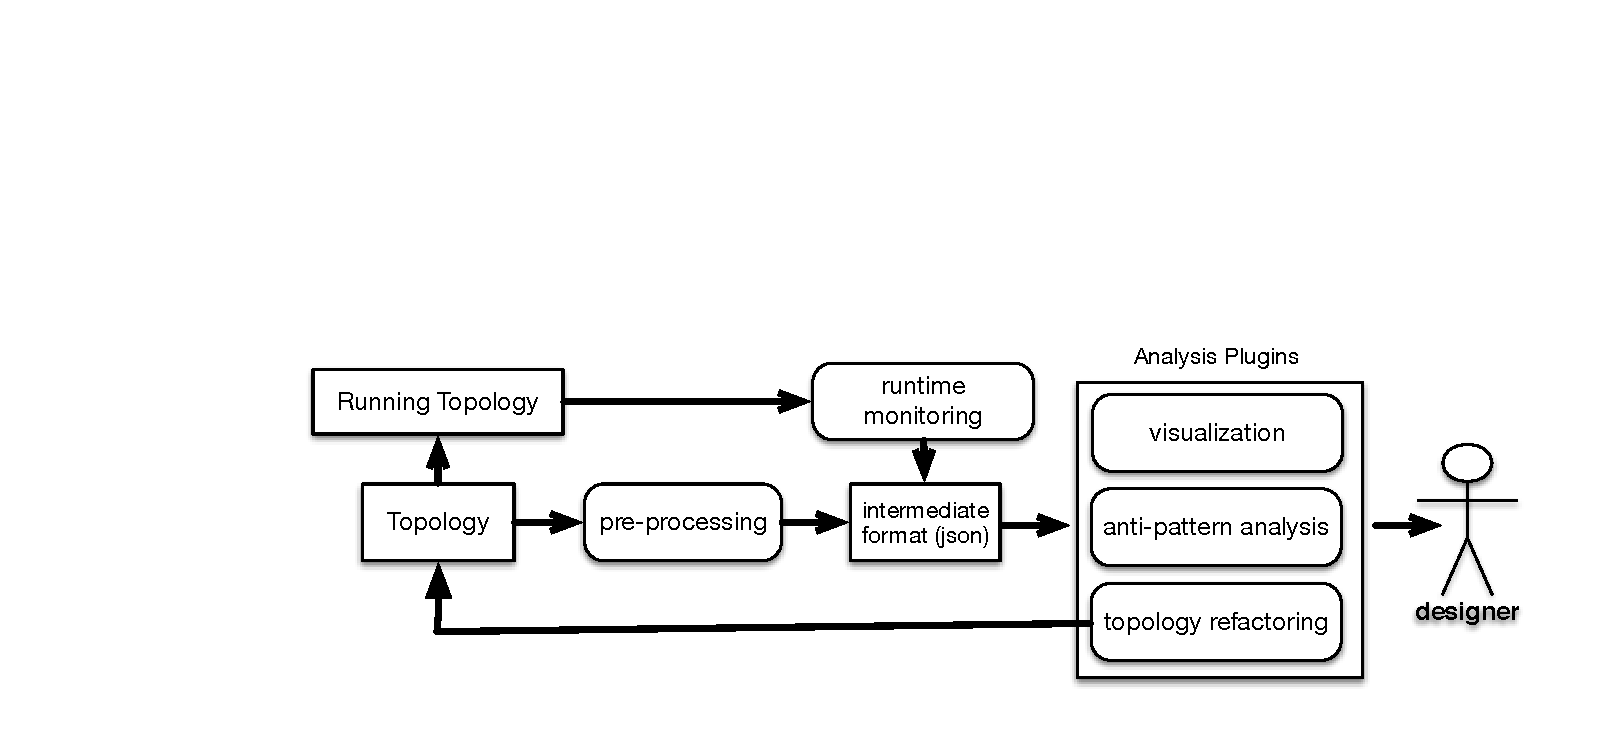
\includegraphics[width=8cm]{images/ostia-arch}
		\caption{OSTIA extensible architecture.}
		\label{fig:ostia-arch}
	\end{center}
\end{figure}


